\section{Evaluation}

We evaluate the implemented algorithm on doth regular and context-free path queries in order to demonstrate applicability of the proposed solution.
Namely, goals of the evaluation are following.
\begin{enumerate}
	\item Investigate practical applicability of RPQ evaluation by the proposed algorithm.
	\item Compare Azimov's algorithm for reachability CFPQ and the proposed algorithm.
	\item Investigate practical applicability of paths extraction algorithm for both regular and context-free queries.
\end{enumerate}

For evaluation, we use a PC with Ubuntu 18.04 installed.
It has Intel core i7-6700 CPU, 3.4GHz, and DDR4 64Gb RAM.
As far as we evaluate only algorithm execution time, we store each graph fully in RAM as its adjacency matrix in sparse format.
Note, that graph loading time is not included in the result time of evaluation.	

\subsection{RPQ Evaluation}

In oder to investigate applicability of the proposed algorithm for RPQ over real-world graphs we collect a set of real-world and synthetic graphs and evaluate queries generated by using the most popular templates for RPQs.

\subsubsection{Dataset}

Brief description of collected graphs are presented in table~\ref{tbl:graphs_for_rpq}.
Namely, the dataset consists of several parts.
The first one is a set of LUBM graphs\footnote{Lehigh University Benchmark (LUBM) web page: \url{http://swat.cse.lehigh.edu/projects/lubm/}. Access date: 07.07.2020.}~\cite{10.1016/j.websem.2005.06.005} with different number of vertices.
The second one is a graphs from Uniprot database\footnote{Universal Protein Resource (UniProt) web page: \url{https://www.uniprot.org/}. All files used for evaluation can be downloaded here: \url{ftp://ftp.uniprot.org/pub/databases/uniprot/current_release/rdf/}. Access date: 07.07.2020.}: \textit{proteomes}, \textit{taxonomy} and \textit{uniprotkb}.
The last part is a RDF files \textit{mappingbased\_properties} from DBpedia\footnote{DBpedia project web site: \url{https://wiki.dbpedia.org/}. Access date: 07.07.2020.} and \textit{geospecies}\footnote{The Geospecies RDF: \url{https://old.datahub.io/dataset/geospecies}. Access date: 07.07.2020.}.
These graphs represents data from different areas and they are frequently used for graph querying algorithms evaluation.

\begin{table}
{
\rowcolors{2}{black!2}{black!10}
\begin{tabular}{|l|c|c|}
\hline
Graph & \#V & \#E \\
\hline
\hline 
LUBM1k  & 120 926 & 484 646 \\
LUBM3.5k  & 358 434 & 144 9711 \\
LUBM5.9k  & 596 760 & 2 416 513 \\
LUBM1M   & 1 188 340 & 4 820 728 \\
LUBM1.7M & 1 780 956 & 7 228 358 \\
LUBM2.3M & 2 308 385 & 9 369 511 \\
\hline
Uniprotkb & 6 442 630 & 24 465 430 \\
Proteomes & 4 834 262 & 12 366 973 \\
Taxonomy & 5 728 398 & 14 922 125 \\
\hline
Geospecies & 450 609 & 2 201 532 \\
Mappingbased\_properties & 8 332 233 & 25 346 359 \\
\hline
\end{tabular}
}
\caption{Graphs for RPQ evaluation}
\label{tbl:graphs_for_rpq}
\end{table}


Queries for evaluation was generated by using templates of the most popular RPQs which are collected from~
\cite{Pacaci2020RegularPQ} (Table 2) and~\cite{Wang2019} (some of complex queries from Table 5), and are presented in table~\ref{tbl:queries_templates}.
We generate 10 queries for each template and each graph using the most frequent relations from the given graph randomly\footnote{Used generator is available as part of CFPQ\_data project: \url{https://github.com/JetBrains-Research/CFPQ_Data/blob/master/tools/gen_RPQ/gen.py}. Access data: 07.07.2020.}. 
For all LUBM graphs common set of queries was generated in order to investigate scalability of the proposed algorithm.

\begin{table}
{\small
\renewcommand{\arraystretch}{1.25}
\rowcolors{2}{black!2}{black!10}
\begin{tabular}{|c|c||c|c|}
\hline

Name & Query & Name & Query \\
\hline
\hline 
$Q_1$   & $a^*$                               & $Q_9^5$    & $(a \mid b \mid c \mid d \mid e)^+$                     \\
$Q_2$   & $a\cdot b^*$                        & $Q_{10}^2$ & $(a \mid b) \cdot c^*$                                  \\
$Q_3$   & $a \cdot b^* \cdot c^*$             & $Q_{10}^3$ & $(a \mid b \mid c)  \cdot d^*$                          \\
$Q_4^2$ & $(a \mid b)^*$                      & $Q_{10}^4$ & $(a \mid b \mid c \mid d)  \cdot e^*$                   \\
$Q_4^3$ & $(a \mid b \mid c)^*$               & $Q_{10}^5$ & $(a \mid b \mid c \mid d \mid e)  \cdot f^*$            \\
$Q_4^4$ & $(a \mid b \mid c \mid d)^*$        & $Q_{10}^2$ & $a \cdot b$                                             \\
$Q_4^5$ & $(a \mid b \mid c \mid d \mid e)^*$ & $Q_{11}^3$ & $a \cdot b \cdot c$                                     \\
$Q_5$   & $a \cdot b^* \cdot c$               & $Q_{11}^4$ & $a \cdot b \cdot c \cdot d$                             \\
$Q_6$   & $a^* \cdot b^*$                     & $Q_{11}^5$ & $a \cdot b \cdot c \cdot d \cdot f$                     \\
$Q_7$   & $a \cdot b \cdot c^*$               & $Q_{12}$   & $(a \cdot b)^+ \mid  (c \cdot d)^+$                     \\
$Q_8$   & $a? \cdot b^*$                      & $Q_{13}$   & $(a \cdot(b \cdot c)^*)^+ \mid  (d \cdot f)^+$          \\
$Q_9^2$ & $(a \mid b)^+$                      & $Q_{14}$   & $(a \cdot b \cdot (c \cdot d)^*)^+  \cdot (e \mid f)^*$ \\
$Q_9^3$ & $(a \mid b \mid c)^+$               & $Q_{15}$   & $(a \mid b)^+ \cdot (c \mid d)^+$                       \\
$Q_9^4$ & $(a \mid b \mid c \mid d)^+$        & $Q_{16}$   & $a \cdot b \cdot (c \mid d \mid e)$                     \\
\hline
\end{tabular}
}
\caption{Queries' templates for RPQ evaluation}
\label{tbl:queries_templates}
\end{table}


\subsubsection{Results}

For reachability index creation average time of 5 runs is presented.

Reachability index creation time for each query for LUBM graphs set is presented in figure~\ref{fig:lubm_all_qs}.
We can observe linear dependency of evaluation time on graph size.
Also we can see, that query evaluation time depends on query: there are queries which evaluate less then 1 second even for biggest graph ($Q_2$, $Q_5$, $Q_{11}^2$, $Q_{11}^3$), while worst time is 6.26 seconds ($Q_{14}$).
Anyway, we can argue that in this case our algorithm demonstrates reasonable time to be applied for real-world data analysis, because it is comparable with recent results on the same problem for LUBM querying by using distributed system over 10 nodes~\cite{Wang2019}, while we use only one node. 
Note, that accurate comparison of different approaches is a huge interesting work for the future.

\begin{figure}
   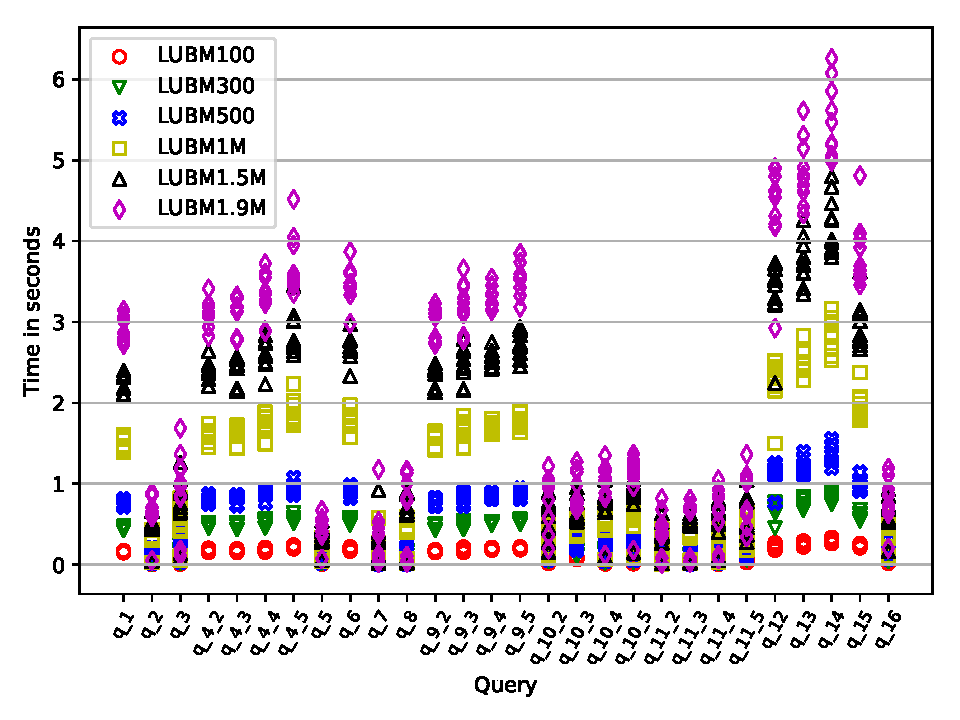
\includegraphics[width=0.48\textwidth]{data/LUBM_all.pdf}
   \caption{Reachability index creation time for LUBM graphs}
   \label{fig:lubm_all_qs}
\end{figure}

Reachability index creation time for each query for for real-world graphs is presented in figure~\ref{fig:other_all_qs}.
We can see that query evaluation time depends on graph inner structure. 
First of all, in some cases handling of small graph requires more time, then handling bigger graph.
For example, $Q_{10}^4$: querying the \textit{geospecies} graph (450k vertices) in some cases requires more time than querying of \textit{mappingbased\_properties} (8.3M vertices) and \textit{taxonomy} (5.7M vertices).
On the other hand, \textit{taxonomy} querying in relatively big number of cases requires significantly more time, than querying of other graphs, while \textit{taxonomy} is not a bigger graph. 
Finally, we can see, that in big number of cases query execution time requires less then 10 seconds, even for big graph, and no queries which require more then 52.17 seconds. 

\begin{figure}
   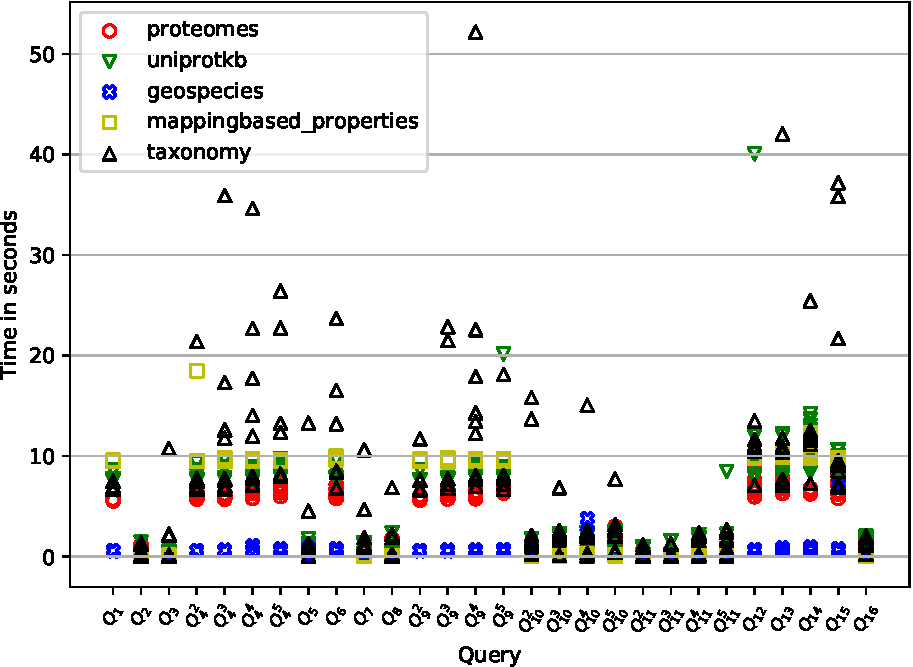
\includegraphics[width=0.48\textwidth]{data/other_all.pdf}
   \caption{Reachability index creation time for real-world RDFs}
   \label{fig:other_all_qs}
\end{figure}

Paths extraction was evaluated on cases with possible long paths.
These cases were selected during reachability index creation by using number of iterations in transitive closure evaluation.
For each selected graph and query we measure paths extraction time for each reachable pair, reachability index creation time is not included because exactly the same index, as calculated at the previous step, is used for paths extraction. 

We evaluate two scenarios.
The first one is a single path extraction.
In this case results are represented as a dependency of extraction time on extracted path length.
We can see linear !!!!

The second scenario is many paths extraction.
Here we limit a number of path to extract by !!! 
In this case results are represented as a dependency of extraction time on number of extracted paths.


\begin{figure}
     \begin{subfigure}[b]{0.24\textwidth}
         \centering
         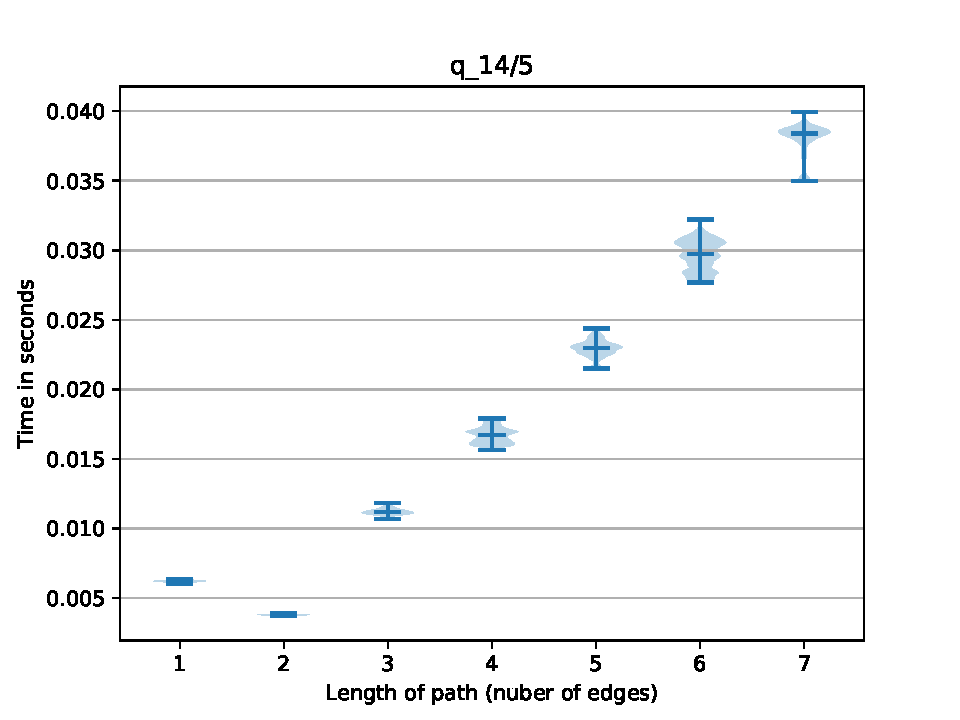
\includegraphics[width=\textwidth]{data/res_graphics/q_14_5.pdf}
         \caption{$y=x$}
         \label{fig:y equals x}
     \end{subfigure}
     ~\begin{subfigure}[b]{0.24\textwidth}
         \centering
         \includegraphics[width=\textwidth]{data/res_graphics/q9_2_8.pdf}
         \caption{$y=x$}
         \label{fig:y equals x}
     \end{subfigure}\\
     \begin{subfigure}[b]{0.24\textwidth}
         \centering
         \includegraphics[width=\textwidth]{data/res_graphics/q_14_8.pdf}
         \caption{$y=x$}
         \label{fig:y equals x}
     \end{subfigure}
     ~\begin{subfigure}[b]{0.24\textwidth}
         \centering
         \includegraphics[width=\textwidth]{data/res_graphics/q4_2_8.pdf}
         \caption{$y=x$}
         \label{fig:y equals x}
     \end{subfigure}
   %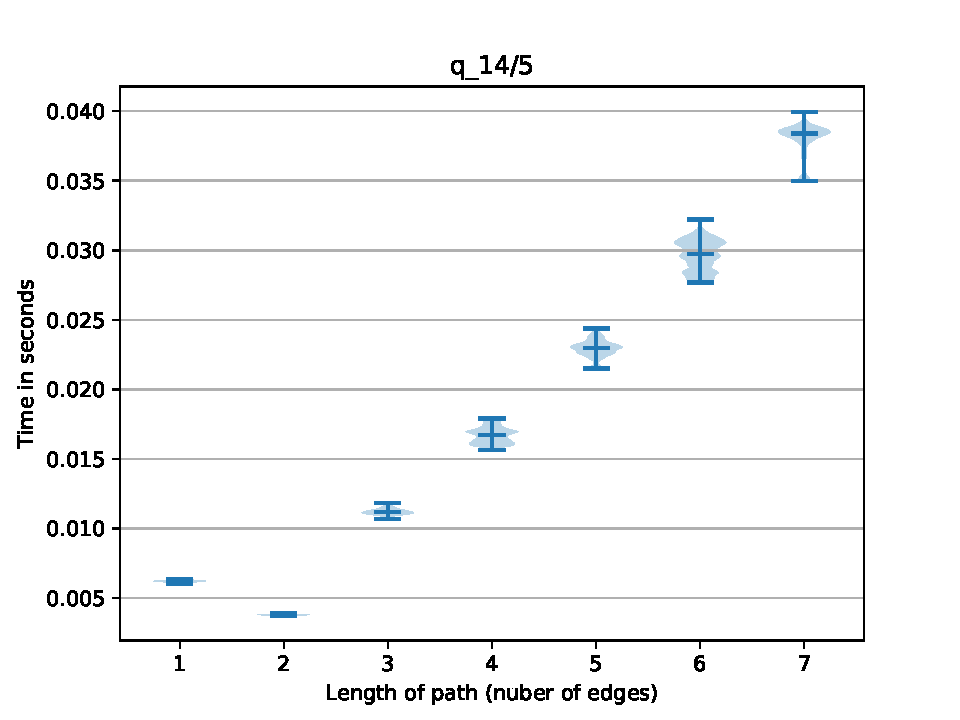
\includegraphics[width=0.48\textwidth]{data/res_graphics/q_14_5.pdf}
   \caption{Single path extraction}
\end{figure}

\subsubsection{Conclusion}

We can conclude that proposed algorithm is applicable for real-world data processing: the algorithm allows one both to solve reachability problem and to extract paths of interest in reasonable time even using na{\"i}ve implementation.  

\subsection{CFPQ Evaluation}

Comparison with matrix-based algorithm.

\subsubsection{Dataset}

Dataset for evaluation. 
It should be CFPQ\_Data\footnote{CFPQ\_Data is a dataset for CFPQ evaluation which contains both synthetic and real-world data and queries \url{https://github.com/JetBrains-Research/CFPQ\_Data}. Access date: 07.07.2020.}

Same-generation queries, memory aliases.

\subsubsection{Results}

Results of evaluation.

Index creation.

Paths extraction.

\subsubsection{Conclusion}
